\documentclass{article}
\usepackage[papersize={6.95in,3.65in},margin=9pt]{geometry}
% Shared visual grammar for FIGURE_FREEZE_V1.
% One blue family + grayscale. Meaning also encoded by shape/border.
\usepackage[T1]{fontenc}
\usepackage{lmodern}
\usepackage{amsmath,amssymb}
\usepackage{tikz}
\usetikzlibrary{arrows.meta,positioning,fit,calc,matrix}

\definecolor{ink}{HTML}{22272B}
\definecolor{muted}{HTML}{5C6770}
\definecolor{rule}{HTML}{B7C0C7}
\definecolor{band}{HTML}{F3F5F7}
\definecolor{accent}{HTML}{2E5A88}
\definecolor{accentfill}{HTML}{E7F0F6}

\tikzset{
  arr/.style={-{Latex[length=2.1mm,width=1.6mm]}, line width=0.6pt, draw=ink},
  arrd/.style={-{Latex[length=2.1mm,width=1.6mm]}, densely dashed, line width=0.6pt, draw=muted},
  figbase/.style={
    font=\small\selectfont,
    color=ink,
    line cap=round,
    line join=round,
  },
  box/.style={
    draw=ink, line width=0.55pt,
    rounded corners=1.4pt,
    inner sep=3.6pt,
    align=center,
    text=ink,
  },
  boxplain/.style={box, fill=white},
  boxband/.style={box, fill=band, draw=rule},
  boxaccent/.style={box, fill=accentfill, draw=accent, line width=0.7pt},
  untrusted/.style={box, densely dashed, draw=muted, fill=white},
  badge/.style={
    font=\footnotesize\selectfont,
    inner sep=2.2pt,
    align=center,
    draw, line width=0.6pt,
    rounded corners=1.1pt,
  },
  badgeexact/.style={badge, fill=accentfill, draw=accent},
  badgesubst/.style={badge, fill=white, draw=accent, densely dashed},
  badgerule/.style={badge, fill=white, draw=ink, double, double distance=1.05pt},
  badgeunk/.style={badge, fill=white, draw=muted, dotted},
  badgerefuse/.style={badge, fill=white, draw=ink, dashed},
  lab/.style={font=\footnotesize\selectfont, text=muted, align=center, inner sep=1pt},
  head/.style={font=\normalsize\bfseries\selectfont, text=accent, align=center},
  axislab/.style={font=\footnotesize\selectfont, text=ink},
}

\pagestyle{empty}
\setlength{\parindent}{0pt}
\begin{document}
\centering
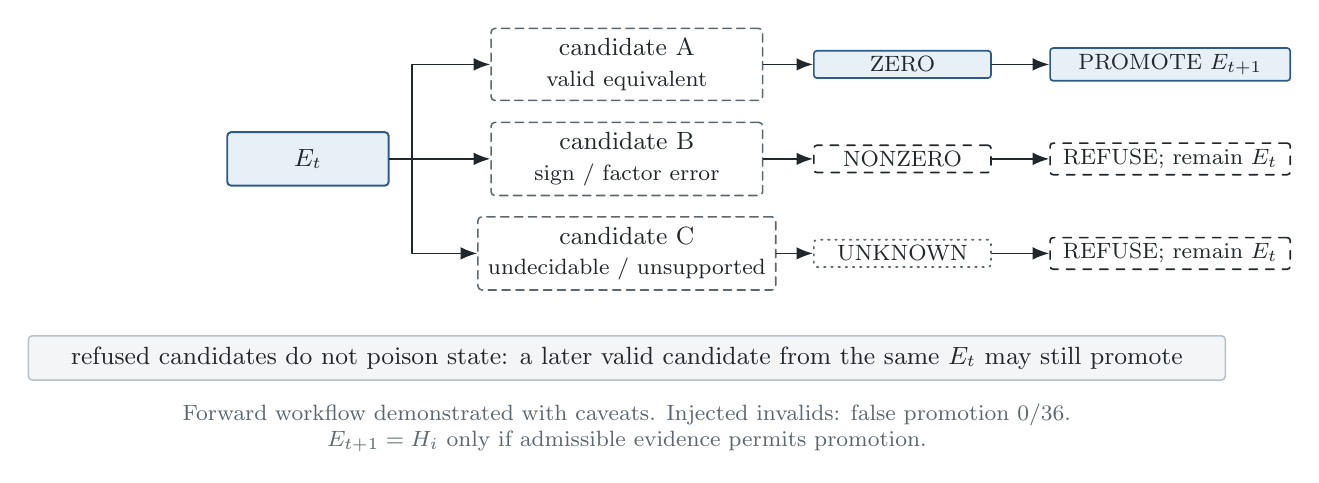
\begin{tikzpicture}[figbase]
  \node[boxaccent, minimum width=2.05cm, minimum height=0.68cm] (et) at (0,1.35) {$E_t$};

  \node[untrusted, minimum width=3.45cm, minimum height=0.82cm] (a) at (4.05,2.55)
    {candidate A\\{\footnotesize valid equivalent}};
  \node[untrusted, minimum width=3.45cm, minimum height=0.82cm] (b) at (4.05,1.35)
    {candidate B\\{\footnotesize sign / factor error}};
  \node[untrusted, minimum width=3.45cm, minimum height=0.82cm] (c) at (4.05,0.15)
    {candidate C\\{\footnotesize undecidable / unsupported}};

  \draw[arr] (et.east) -- ++(0.28,0) |- (a.west);
  \draw[arr] (et) -- (b);
  \draw[arr] (et.east) -- ++(0.28,0) |- (c.west);

  \node[badgeexact, minimum width=2.25cm] (za) at (7.55,2.55) {ZERO};
  \node[badgerefuse, minimum width=2.25cm] (zb) at (7.55,1.35) {NONZERO};
  \node[badgeunk, minimum width=2.25cm] (zc) at (7.55,0.15) {UNKNOWN};
  \draw[arr] (a) -- (za);
  \draw[arr] (b) -- (zb);
  \draw[arr] (c) -- (zc);

  \node[badgeexact, minimum width=3.05cm] (pa) at (10.95,2.55) {PROMOTE $E_{t+1}$};
  \node[badgerefuse, minimum width=3.05cm] (pb) at (10.95,1.35) {REFUSE; remain $E_t$};
  \node[badgerefuse, minimum width=3.05cm] (pc) at (10.95,0.15) {REFUSE; remain $E_t$};
  \draw[arr] (za) -- (pa);
  \draw[arr] (zb) -- (pb);
  \draw[arr] (zc) -- (pc);

  \node[boxband, below=16pt of c, minimum width=15.2cm, align=center, inner sep=4pt] (rec)
    {refused candidates do not poison state: a later valid candidate from the same $E_t$ may still promote};

  \node[lab, below=7pt of rec, align=center]
    {Forward workflow demonstrated with caveats.
     Injected invalids: false promotion $0/36$.\\
     $E_{t+1}=H_i$ only if admissible evidence permits promotion.};
\end{tikzpicture}
\end{document}
